\documentclass{article} % For LaTeX2e
\usepackage{nips13submit_e,times}
\usepackage{hyperref}
\usepackage{url}
\usepackage{textcomp}
\usepackage[utf8]{inputenc}
\usepackage{array}
\usepackage{amsmath}
\usepackage{pgfplots}
\usepackage{caption}
\usepackage{adjustbox} 
\usepackage{graphicx}
\usepackage{algorithm}
\usepackage{algpseudocode}

\title{Sparse Coding and Unsupervised Feature Ensembling}

\author{
Gabriel Forgues \\
\texttt{gabriel.forgues@mail.mcgill.ca} \\
\And 
Benedicte Leonard-Cannon \\
\texttt{benedicte.leonard-cannon@mail.mcgill.ca} \\
}
\nipsfinalcopy

\begin{document}
\maketitle

\section{Introduction}
There has been a significant research effort in recent years to develop algorithms to extract good features from unlabelled data. Three of these methods that are often used in the literature include denoising autoencoders, restricted Boltzmann machines (RBMs), and sparse coding. These three approaches have very different training objectives, but they can all be used to extract features in an unsupervised way. Due to their different training objectives, intuition would suggest that they might not learn identical features. In many machine learning tasks, it has also been shown that ensemble methods which combine predictions of many different classifiers can outperform a single classifier. In this project, we investigate whether combining features from different unsupervised learning algorithms, which we refer to as feature ensembling, can be beneficial as well. We first compare the performances of a classifier trained on three different sets of features, each extracted with a different unsupervised learning algorithm (denoising autoencoders, RBMs, and sparse coding). Then, we compare these results with a classifier trained on combinations of features from the three learning algorithms. We take our own previous implementations of denoising autoencoders and RBMs, which we use as two comparable baselines. We then experiment with our own implementation of a sparse coding algorithm, and compare its performance as a stand-alone set of features or in feature combinations against the two baselines. We evaluate the effectiveness of the different models on a handwritten letter recognition task. Since the data is composed of very simple but distinct shapes, it is well suited for a sparse code algorithm. Indeed, we would expect the sparse code to learn visually interpretable dictionary features (i.e. letter strokes) which help us validate the correctness of our implementation.

\section{Sparse coding}
Sparse coding is a method which aims to learn a dictionary of features in such a way that inputs can be represented as a sparse combination of these features. This is in contrast to RBMs and denoising autoencoders where, although regularization can be incorporated into their learning algorithms, are not explicitly designed to induce sparse representations.

As is the case for RBMs and autoencoders, sparse coding is an unsupervised learning algorithm which learns features solely from unlabeled data. The intuition behind the algorithm can be more readily understood from the perspective of human vision. When considering the set of all possible images, a large majority of these would appear to humans simply as noise with no inherent structure. The subset of natural images is a very small fraction of all possible images, and humans can easily recognize them from the way they are distinctly structured. We can decompose natural images into a set of common structures. For example, a door would be composed of two parallel horizontal edges, two parallel vertical edges, and perhaps a round doorknob. The doorknob could be further decomposed into a set of slightly curved edges, joined together in the shape of a circle. Although there might exist a large amount of structural components in the set of all natural images, any given image would only contain a few of these structural components. Sparse coding aims to build a dictionary of these common structures, and represent each natural image as a sparse composition of these structures. By enforcing a strong sparsity constraint, we ensure that each image can be adequately represented by a very small number of these structures. The sparsity might then favour the extraction of more high-level features which are dense in meaning compared to more low-level features such as Gabor filters.

\subsection{Training objective}
More formally, we denote $D$ the dictionary of features and $h(x)$ as the sparse representation of input $x$ which uses $D$ as a basis.

Then, the training objective is given as:

\begin{equation}
\min_{D} \frac{1}{T} \sum_{t=1}^{T} \min_{h^{(t)}} \frac{1}{2} \Vert x^{(t)} - D h^{(t)} \Vert_{2}^{2} + \lambda \Vert h^{(t)} \Vert_{1}
\end{equation}

The first term is the reconstruction loss, which the training objective aims to minimize. The second term is the sparsity constraint on $h$, with an L1 regularization coefficient of $\lambda$.

\subsection{Inference with ISTA}
However, inferring a sparse representation $h^{(t)}$ for an input $x^{(t)}$ given a dictionary $D$ is now a complication function:

\begin{equation}
h(x^{(t)}) = \arg\min_{h^{(t)}} \frac{1}{2} \Vert x^{(t)} - D h^{(t)} \Vert_{2}^{2} + \lambda \Vert h^{(t)} \Vert_{1}
\end{equation}

We must perform gradient descent to find the optimal $h^{(t)}$. To do this, we start by taking the regularized reconstruction loss for a given input:
\begin{equation}
l(x^{(t)}) = \frac{1}{2} \Vert x^{(t)} - D h^{(t)} \Vert_{2}^{2} + \lambda \Vert h^{(t)} \Vert_{1}
\end{equation}

And then take the derivative with respect to $h^{(t)}$:

\begin{equation}
\nabla_{h^{(t)}} l (x^{(t)}) = D^T(D h^{(t)}) + \lambda \text{sign} (h^{(t)})
\end{equation}

But since the L1 norm is not differentiable at 0, we use the Iterative Shrinkage and Thresholding Algorithm (ISTA) instead. The ISTA algorithm alternates between a step along the gradient of $h^{(t)}$, and a shrinkage to $0$ if $h^{(t)}$ is within a threshold distance $\alpha\lambda$ from $0$. This ensures that, although the gradient is non-differentiable at 0, the algorithm will converge instead of oscillating between a large positive or a large negative step when close to $0$.

\begin{algorithm}
\caption{Iterative Shrinkage and Thresholding Algorithm (ISTA)}
\begin{algorithmic}[1]
\State $h^{(t)}\gets $ zero vector
\State $h'^{(t)}\gets $ non-zero vector \Comment{$h'$ will store stepwise updates of $h$}
\While{$|h^{(t)} - h'^{(t)}| > \epsilon$}\Comment{$\epsilon$ is the convergence threshold}
	\State $h^{(t)}\gets h'^{(t)}$
	\State $h'^{(t)}\gets h^{(t)} - \alpha D^T(Dh^{(t)} - x^{(t)})$ \Comment{$\alpha$ is the learning rate}
	\State $h'^{(t)}\gets \text{sign}(h'^{(t)}) \text{max}(|h'^{(t)}| - \alpha\lambda, 0)$ \Comment{$\lambda$ is the L1 regularization term}
\EndWhile
\State\Return $h^{(t)}$
\end{algorithmic}
\end{algorithm}

\subsection{Dictionary learning}
With ISTA, we can infer $h^{(t)}$ for each $x^{(t)}$ given a dictionary $D$. However, the dictionary $D$ must also be learned. We update the dictionary with block-coordinate gradient descent. We refer to the class notes for the full derivation\footnote{Block-coordinate dictionary update: \url{https://dl.dropboxusercontent.com/u/19557502/8_04_dictionary_update_block-coordinate_descent.pdf}}, and instead give the two results which we will use to apply column-wise gradient updates to the dictionary.

\begin{equation}
A = \sum_{t=1}^T h(x^{(t)}) h(x^{(t)})^T
\end{equation}
\begin{equation}
B = \sum_{t=1}^T x^{(t)} h(x^{(t)})^T
\end{equation}


The dictionary learning proceeds with two alternating steps. First, we randomly initialize the dictionary $D$ and infer a sparse representation $h^{(t)}$ for each input $x^{(t)}$ by performing ISTA until convergence. Then, we take steps along the gradient for each column $D_{.,j}$ until convergence. We then repeat the $h^{(t)}$ inference and dictionary update steps for some fixed number of epochs, at which point the dictionary will have converged to a good basis for sparse representations of the data.


\begin{algorithm}
\caption{Batch dictionary update with block-coordinate descent}
\begin{algorithmic}[1]
\State $D\gets$ random initialization
\While{$D$ has not converged} 
	\For{each $x^{(t)}$}
		\State infer $h^{(t)}$ \Comment{inference done with ISTA}
	\EndFor
	\State compute A, B using equations (5) and (6) above
	\While{$D$ has not converged}
		\For{each column $D_{.,j}$}
			\State $D_{.,j}\gets \frac{1}{A_{j,j}} (B_{.,j} - D A_{.,j} + D_{.,j} A_{j,j})$
			\State $D_{.,j}\gets \frac{D_{.,j}}{\Vert D_{.,j} \Vert_2}$ \Comment{normalization step}
		\EndFor
	\EndWhile
\EndWhile
\State\Return $D$
\end{algorithmic}
\end{algorithm}

\section{Classifier architecture}
We wish to compare the effectiveness of three unsupervised learning algorithms. To do so, we train the same classifier on the set of features extracted from each unsupervised learning algorithm, or combinations of these sets of features. We use a support vector machine (SVM) with an RBF kernel (implemented by scikit-learn\footnote{Scikit-learn: \url{scikit-learn.org}} as a good general-purpose classifier in all feature comparisons.

\subsection{Feature extraction}
Once all the unsupervised learning algorithms have been trained, we can use them to extract features from some input $x$. The feature extraction process is the same for RBMs and autoencoders, and can be viewed as a single hidden layer feed-forward neural network. Although their training objectives differ, both RBMs and autoencoders effectively learn a set of weights $W$ and biases $b$ to connect a set of inputs to a set of hidden units. Given the learned set of weights $W$ and biases $b$, we extract features by applying a standard feed-forward propagation:
\begin{equation}
h(x) = \text{sigmoid}(W^T x + b)
\end{equation}
The values of the hidden layer are then used as input features to the classifier.

For the sparse coding algorithm, feature extraction proceeds as described in the ISTA algorithm. We infer a sparse representation $h(x)$ using the learned dictionary $D$, and then use this sparse $h(x)$ as features for the classifier.

For all experiments, we use the pre-defined data splits from the OCR letters dataset, with $32,152$ training, $10,000$ validation and $10,000$ test images. The experimental pipeline works as follows. We first train each unsupervised learning algorithm independently (i.e. RBM, autoencoder and sparse coding). We select hyper-parameters for each model based on its performance on a validation set. However, because the sparse coding algorithm is very slow (especially due to ISTA), we do the hyper-parameter search on a subset of only 1,000 training images. We then use the best hyper-parameters for each model to extract features from the data, and compare the effectiveness of the features extracted by each algorithm. Although our hyper-parameter exploration considers varying the number of hidden units (i.e. number of features) to evaluate its impact on validation accuracy, we ignore this hyper-parameter when comparing unsupervised algorithms. Instead, when we compare the performance between different algorithms (independently or in combinations), we fix the number of hidden units to be the same for all models to ensure a fair comparison. Finally, we train SVMs all these sets of features, this time using the entire training set, and then evaluate their performance on the test set.

\section{Results}
\subsection{Hyperparameter optimization}
\begin{table}[h]
\caption{Average training and validation accuracy for denoising autoencoder hyper-parameter
 search using a training subset of size 1000}
\label{results-table}
\begin{center}
\begin{adjustbox}{width=1\textwidth}
\begin{tabular}{cccc|rr}

\multicolumn{1}{c}{\bf Learning rate}  
&\multicolumn{1}{c}{\bf \# Hidden units}  
&\multicolumn{1}{c}{\bf \# Epochs} 
&\multicolumn{1}{c}{\bf Noise prob.} 
&\multicolumn{1}{|r}{\bf Accuracy (train.)}
&\multicolumn{1}{r}{\bf Accuracy (valid.)}
\\ \hline \\	
0.01 & 50 & 10 & 0.3 & 0.684 & 0.587 \\
0.01 & 50 & 10 & 0.5 & 0.621 & 0.554 \\
0.01 & 50 & 10 & 0.1 & 0.720 & 0.603 \\
0.01 & 30 & 10 & 0.1 & 0.707 & 0.606 \\
0.01 & 70 & 10 & 0.1 & 0.714 & 0.602 \\
0.01 & 140 & 10 & 0.1 & 0.699 & 0.592 \\
0.01 & 30 & 5 & 0.1 & 0.707 & 0.596 \\
0.01 & 30 & 15 & 0.1 & 0.712 & 0.610 \\
0.05 & 30 & 15 & 0.1 & 0.714 & \textbf{0.619} \\
0.01 & 30 & 15 & 0.1 & 0.722 & 0.599 \\

\end{tabular}
\end{adjustbox}
\end{center}
\end{table}


\begin{table}[h]
\caption{Average training and validation accuracy for RBM hyper-parameter
 search using a training subset of size 1000}
\label{results-table}
\begin{center}
\begin{adjustbox}{width=1\textwidth}
\begin{tabular}{cccc|rr}

\multicolumn{1}{c}{\bf Learning rate}  
&\multicolumn{1}{c}{\bf \# Hidden units}  
&\multicolumn{1}{c}{\bf \# Epochs} 
&\multicolumn{1}{c}{\bf \# CDk} 
&\multicolumn{1}{|r}{\bf Accuracy (train.)}
&\multicolumn{1}{r}{\bf Accuracy (valid.)}
\\ \hline \\	
0.01 & 50 & 10 & 3 & 0.685 & \textbf{0.611} \\
0.01 & 70 & 10 & 3 & 0.670 & 0.595 \\
0.01 & 30 & 10 & 3 & 0.676 & 0.581 \\
0.01 & 50 & 5 & 3 & 0.644 & 0.575 \\
0.01 & 50 & 15 & 3 & 0.687 & 0.606 \\
0.01 & 50 & 10 & 1 & 0.665 & 0.600 \\
0.01 & 50 & 10 & 5 & 0.667 & 0.583 \\
0.05 & 50 & 10 & 3 & 0.629 & 0.558 \\
0.005 & 50 & 10 & 3 & 0.669 & 0.593 \\
0.01 & 60 & 10 & 3 & 0.695 & 0.599 \\

\end{tabular}
\end{adjustbox}
\end{center}
\end{table}


\begin{table}[h]
\caption{Average training and validation accuracy for sparse coding hyper-parameter
 search using a training subset of size 1000}
\label{results-table}
\begin{center}
\begin{adjustbox}{width=1\textwidth}
\begin{tabular}{cccc|rr}

\multicolumn{1}{c}{\bf Learning rate}  
&\multicolumn{1}{c}{\bf \# Hidden units}  
&\multicolumn{1}{c}{\bf \# Epochs} 
&\multicolumn{1}{c}{\bf L1} 
&\multicolumn{1}{|r}{\bf Accuracy (train.)}
&\multicolumn{1}{r}{\bf Accuracy (valid.)}
\\ \hline \\	
0.1 & 50 & 5 & 0.1 & 0.936 & 0.509 \\
0.1 & 30 & 5 & 0.1 & 0.946 & 0.465 \\
0.1 & 70 & 5 & 0.1 & 0.934 & 0.573 \\
0.1 & 50 & 5 & 0.05 & 0.986 & 0.544 \\
0.1 & 70 & 5 & 0.05 & 0.983 & 0.627 \\
0.1 & 50 & 5 & 0.2 & 0.824 & 0.452 \\
0.2 & 50 & 5 & 0.05 & 0.986 & 0.530 \\
0.05 & 50 & 5 & 0.05 & 0.981 & 0.566 \\
0.1 & 50 & 10 & 0.05 & 0.984 & 0.541 \\
0.1 & 100 & 5 & 0.05 & 0.957 & \textbf{0.630} \\

\end{tabular}
\end{adjustbox}
\end{center}
\end{table}

From the results in Tables 1 to 3, we first notice that the sparse coding algorithm seems much more sensitive to hyper-parameter selection than the two other algorithms. We obtained validation set accuracies as low as 45.2\% and as high as 63\%. Sparse coding also seems more susceptible to overfitting, which we notice from the fact that training set accuracies are much higher than the validation set (up to 98.6\%). Of course, these results are on a very small subset of the entire training data ($1,000$ out of $32,152$) due to the algorithm's slow training time. We would expect overfitting to be less of a problem when using the entire training set. As might be expected, we also find that increasing the capacity of the sparse representation leads to higher accuracy. Somewhat surprisingly, we obtained better results from relaxing the L1 sparsity constraint.
\begin{figure}
\centering
%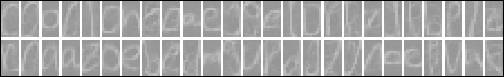
\includegraphics[scale=1]{figures/filters_50.png}
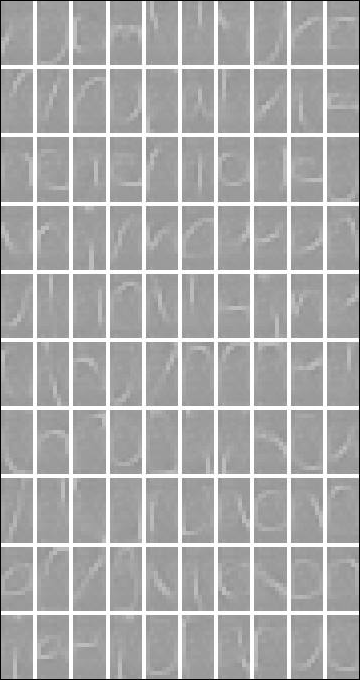
\includegraphics[scale=0.577]{figures/filters_100_clean.png}
\quad\quad\quad
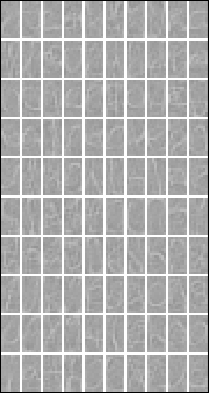
\includegraphics[scale=1]{figures/filters_100_noisy.png}
\caption{Sparse code dictionary filters learned with L1=0.1 (left) or L1=0.05 (right). Although the features learned from a higher regularization constant are more visually distinct, the noisier filters produced slightly higher classification accuracy}
\end{figure}

\begin{figure}
\centering
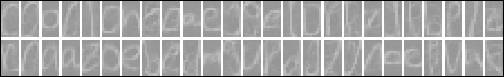
\includegraphics[scale=1]{figures/filters_50.png}
\caption{Sparse code dictionary filters with fewer features and higher regularization (L1=0.2). The features are more high-level and often represent distinct letters.}
\end{figure}

In Figure 1, we compare the dictionary filters learned from different L1 regularization constants. We can see that the higher sparsity constraint of L1=0.1 causes the dictionary to learn clearly visible letter strokes. We can notice features of vertical strokes, as well as many differently oriented curved strokes. We can also see high-level features which represent the entire letter (e.g. the second column contains the letter "e" and "a"). The same figure also shows filters learned with a lower sparsity constraint of L1=0.05. As might be expected, relaxing the sparsity constraint caused the dictionary to learn significantly noisier filters. However, it was surprising that these noisier features produced better classification accuracy. This might be explained by the fact that relaxing the sparsity constraint makes it much easier to learn good reconstructions of the input. The resulting dictionary might not be as visually appealing, but it might fit the data better. In Figure 2, we increase the sparsity constraint even higher to L1=0.2 and learn fewer features, hoping to find many distinct letters. We again notice simple vertical or rounded strokes, but also find many letters of different shapes and sizes ("a", "e", "p", "z", to name a few).


\subsection{Results from ensembling unsupervised feature extractors}
With the visual confirmation that we are learning sensible features, we then compared the performance of an SVM trained on the different types of unsupervised features. In Table 4, we can see that the autoencoder, RBM and sparse coding approaches all produce nearly identical accuracy on the test set when trained with 300 features each (i.e. 300 hidden units in each model). However, an SVM trained on the combination of 100 features from each model performed significantly better compared to features from a single model (86.8\% vs ~83\%). However, the benefit of combining pairs of models was not as clear-cut. Combining sets of 150 features from two out of the three models performed better in two cases and worse in one case when compared to the single feature extractors. Finally, we were surprised to find that an SVM trained on 300 features from each model (therefore 3x as many features as all previous comparisons) did not perform the best.

Our results suggest that, for some fixed number of features, it is better to take a third of all features from each of three different unsupervised learning algorithms rather than take all features from a single one. This leads us to believe that the three learning algorithms are sufficiently different to extract different features whose combination can be beneficial. However, having more features is not always better. The number of features to extract still requires some tuning to obtain optimal results. This might be due to the RBF SVM classifier which might have difficulty handling a larger number of features.




\begin{table}[h]
\caption{Average train and test accuracy based on model combinations}
\label{results-table}
\begin{center}
\begin{adjustbox}{width=1\textwidth}
\begin{tabular}{ccc|rr}

\multicolumn{1}{c}{\bf \# Autoencoder features}  
&\multicolumn{1}{c}{\bf \# RBM features}  
&\multicolumn{1}{c}{\bf \# Sparse coding features} 
&\multicolumn{1}{|r}{\bf Accuracy (train)}
&\multicolumn{1}{r}{\bf Accuracy (test)}
\\ \hline \\	
300 & 0 & 0 & 0.838 & 0.833 \\
0 & 300 & 0 & 0.837 & 0.836 \\
0 & 0 & 300 & 0.854 & 0.830  \\
100 & 100 & 100 & 0.897 & \textbf{0.868} \\
150 & 150 & 0 & 0.850 & 0.807 \\
150 & 0 & 150 & 0.885 & 0.857 \\
0 & 150 & 150 & 0.883& 0.849 \\
300 & 300 & 300 & 0.859 & 0.845 \\

\end{tabular}
\end{adjustbox}
\end{center}
\end{table}

\end{document}